%% ----------------------------------------------------------------------------
% BIWI SA/MA thesis template
%
% Created 09/29/2006 by Andreas Ess
% Extended 13/02/2009 by Jan Lesniak - jlesniak@vision.ee.ethz.ch
%% ----------------------------------------------------------------------------
\newpage
\chapter{Materials and Methods}
The objectives of the ``Materials and Methods'' section are the following:
\begin{itemize}
    \item \textit{What are tools and methods you used?} Introduce the environment, in which your work has taken place - this can be a software package, a device or a system description. Make sure sufficiently detailed descriptions of the algorithms and concepts (e.g. math) you used shall be placed here.
    \item \textit{What is your work?} Describe (perhaps in a separate chapter) the key component of your work, e.g. an algorithm or software framework you have developed.
\end{itemize}


\section{Generative Machine Learning}
\section{Excursion to Bayes}
Before getting started we need to quickly define the terms used in the next section, since they all stem from Bayesian
statistics. The Bayesian theorem can be written like this:
\begin{equation}
    p(z|x) = \frac{p(x|z)p(z)}{p(x)}
\end{equation}
It is implicitly assumed here that $p$ is a probability density function over two continuous random variables $x$ and $z$.
The formula holds in general, but in generative machine learning we usually assume that $z$ represents a random variable in
latent space (unobserved) from which we will eventually sample to generate new samples, whereas $x$ is the random variable that
represents the training images (observed space).
Using above described ordering, the four terms in this formula use distinct names:
\begin{description}
    \item[$p(z|x)$] is called the \textit{posterior}
    \item[$p(x|z)$] is called the \textit{likelihood}, since it gives the literal likelihood of observing an example $x$ when
        choosing the latent space to be a specific $z$.
    \item[$p(z)$] is called the \textit{prior}, since it exposes information on $z$ before any conditioning.
    \item[$p(x)$] is called the \textit{evidence}, since it encompasses our actual observations.
\end{description}
One of the most straightforward examples of a generative model where we search for such a latent space representation of
our distribution over the training examples, is the Variational Autoencoder (VAE)~\autocite{kingma2022autoencoding}. The name of the VAE stems from the Autoencoder,
a network that tries to recreate its output through a bottleneck and thereby learning a compressed representation of the data.~\autocite{https://doi.org/10.1002/aic.690370209}
It bears similarity to other dimension reduction methods like Principal Component Analysis (PCA) and therefore was first published under the name
\textit{Nonlinear principal component analysis}. The \textit{variational} part in the VAE stems from the fact that it tries to reduce the data not into
an arbitrary low dimensional latent space, but into a latent parameterized distribution (usually i.i.d multivariate Gaussian). This distribution is sampled
in the forward pass (therefore \textit{variational}, since we use a stochastic layer) and reproducing the input is now not a feasible loss function, but
maximizing the likelihood is. Maximizing the likelihood $p(x|z)$ from above means that we want to tune the parameters of this latent distribution such that the produced
output is \enquote{likely} an example that could come from the original distribution. Training generative models such as a VAE or also a GAN is usually either done with \textit{Evidence Lower Bound} as the loss, or with an additional network and an \textit{adversarial loss}.~\autocite{goodfellow2014generative} Both examples will be further explained in the next sections.

\section{Loss Functions}
In generative machine learning we would want our model to learn the distribution that generated
out training examples. Often this distribution is conditioned on some description (e.g. text) or
on the corruption process in our case, where we use generative models to solve inverse problems.
Assuming our original data distribution (of images) is $p(x)$, then we try to find a parameterized
variational machine learning model ($q_{\theta}(x)$) that will closely match the data distribution.

In order for this $q_{\theta}(x)$ to be trained we need a differentiable loss function that expresses
\enquote{closeness} in a distributional sense. The usual approach to this is to use the Kullback-Leibler (KL)
divergence.

\subsection{Kullback-Leibler Divergence}

\subsection{Wasserstein Distance}
A different approach to comparing the similarity of distributions is the Wasserstein metric, successfully used in the Wasserstein GAN.~\autocite{arjovsky2017wasserstein}.

\section{Diffusion Denoising Probabilistic Models}
Diffusion Denoising Probabilistic Models (DDPMs or Diffusion Models) are a generative model that learn the distribution of images in a training set. During training, sample images are gradually destroyed by adding noise over many iterations and a neural network is trained, such that these steps can be inverted.

As the name suggests, image content is diffused in timesteps, therefore we use the random variable $\bm{x}_0$ to represent our original training images, $\bm{x}_t$ for (partially noisy) images at an intermediate timestep and $\bm{x}_T$ for images at the end of the process where almost all information has been destroyed and the distribution $q(\bm{x}_T)$ largely follows an isotropic Gaussian distribution -- a Gaussian distribution with the identity matrix as covariance matrix, but a non-zero means vector.

Once our network is trained to create a less noisy image $\bm{x}_{t-1}$ from $\bm{x}_t$, we should be able to sample some new $\bm{x}_T$ and generate new samples from our training distribution $q(\bm{x}_0)$ by passing it many times through our network until all noise is removed.

\subsection{Forward Diffusion Process}
\subsubsection{Mathematical Description}
In order to derive a training objective it is important to understand the workings of the \textit{forward diffusion process}. During this process, i.i.d (independent and identically distributed) Gaussian noise is applied to the image over many discrete timesteps. A \textit{variance schedule} defines the means at variances ($\sqrt{1-\beta}$ and $\beta$) of the added noise at every timestep.~\autocite{ho2020denoising} The whole process can be expressed as a Markov chain (depicted in Fig.~\ref{fig:forward_diffusion})
\begin{equation}
    q(\bm{x}_T|\bm{x}_0) = q(\bm{x}_0) \prod_{t=1}^{T} q(\bm{x}_{t}|\bm{x}_{t-1})
\end{equation}
with the transition distributions $q(\bm{x}_t|\bm{x}_{t-1}) = \mathcal{N}(\sqrt{1-\beta_t} \bm{x}_{t-1}, \beta_t I)$. An example of iterative destruction of an image by this process is shown in Fig.~\ref{fig:forward_naoshima}

\begin{figure}[h]
    \centering
    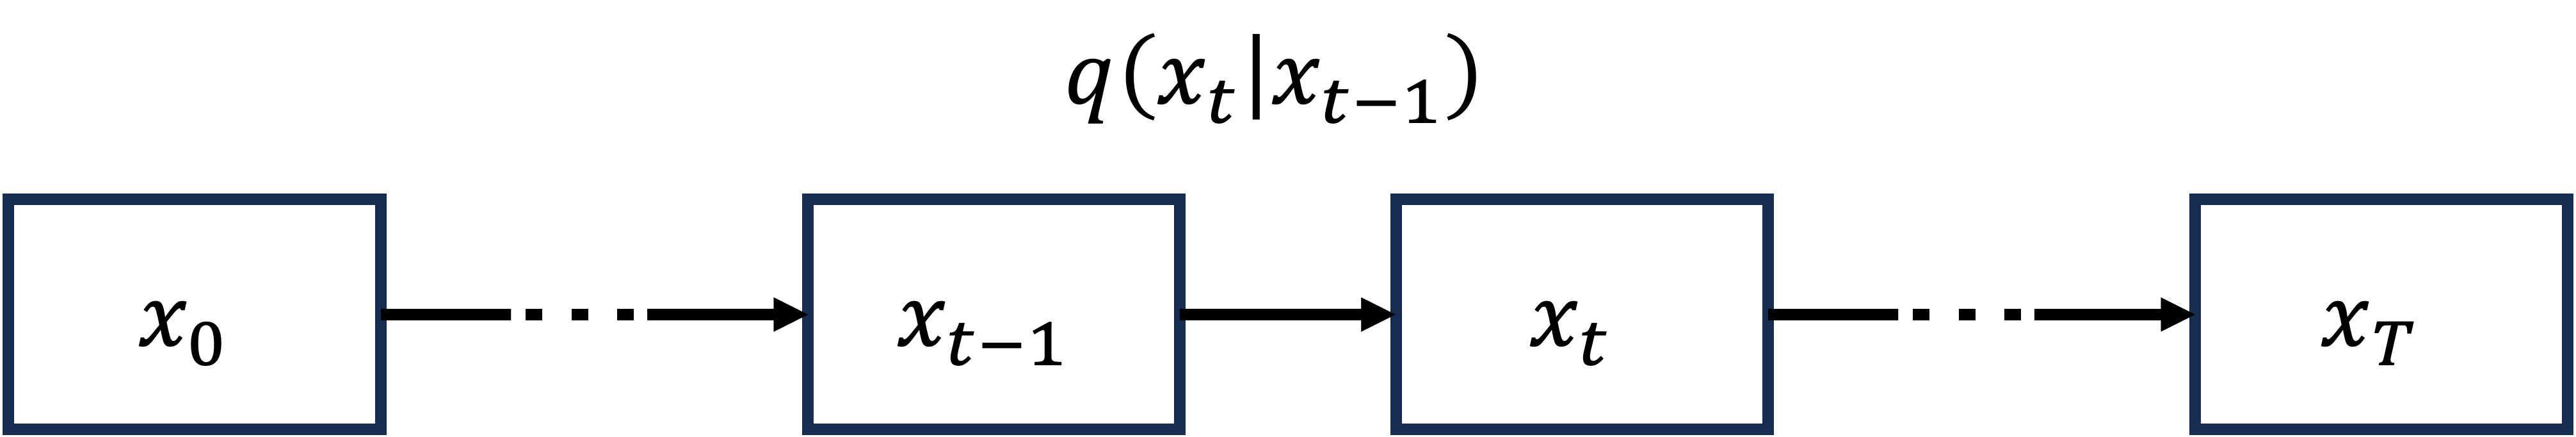
\includegraphics[width=.5\textwidth]{images/forward_diffusion.png}
    \caption{Forward Diffusion Process: An image is iteratively destroyed by adding normally distributed noise,
        according to a schedule. This represents a Markov process with the transition probability $q(\bm{x}_t|\bm{x}_{t-1})$.}
    \label{fig:forward_diffusion}
\end{figure}

\begin{figure}[h]
    \centering
    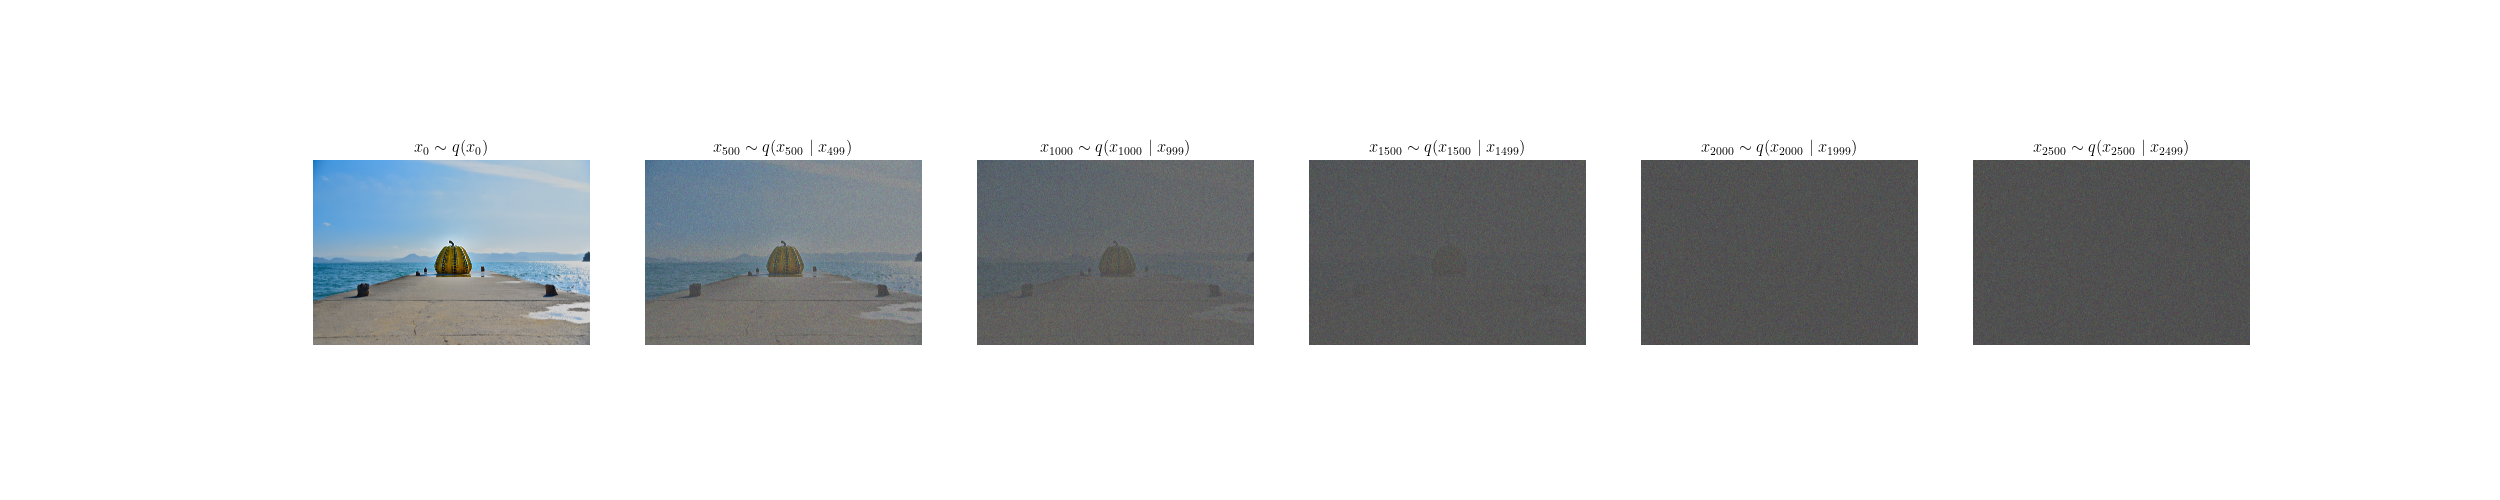
\includegraphics[width=\textwidth]{images/forward_naoshima.png}
    \caption{Example of Iterative Image Destruction through Forward Diffusion Process:
        The indices give the time step in the iterative destruction process, where $\beta$ was created according to a linear noise variance schedule (5000 steps from in the 0.001 to 0.02 range and picture resolution of 4016 by 6016 pixels).}
    \label{fig:forward_naoshima}
\end{figure}

Gladly it is not necessary to sample noise again and again in order to arrive at $\bm{x}_t$, since Ho et al. derived a closed-form solution to the sampling procedure.~\autocite{ho2020denoising} For this, the variance schedule is first reparameterized as $1-\beta = \alpha$
\begin{equation}
    q(\bm{x}_t | \bm{x}_{t-1}) = \mathcal{N}(\sqrt{\alpha_t} \bm{x}_{t-1}, (1-\alpha_t) \bm{I})
    \label{eq:forward_alpha}
\end{equation}
and the closed-form solution for $q(\bm{x}_t|\bm{x}_0)$ is derived by introducing the cumulative product $\bar{\alpha_t} = \prod_{s=1}^{t}\alpha_s$ as
\begin{equation}
    q(\bm{x}_t|\bm{x}_0) = \mathcal{N}(\sqrt{\bar{\alpha_t}}\bm{x}_0, (1-\bar{\alpha_t})\bm{I})
    \label{eq:forward_alphadash}
\end{equation}
The derivation that leads from Eq.~\ref{eq:forward_alpha} to Eq.~\ref{eq:forward_alphadash} will be left to~\ref{app:forward}.

\subsubsection{Influence of Scheduling Functions}
The process of information destruction is dependent on the chosen variance schedule, the number of steps and the image size. Beyond the most simple case -- a constant variance over time -- Ho et al. opted for the second most simple option, a linear schedule, where the variance $\beta_t$ grows linearly in $t$.~\autocite{ho2020denoising} Nichol et al. later found that a cosine-based schedule gives better results, since it does not destruct information quite as quickly, making it more informative in the last few timesteps.~\autocite{nichol2021improved} Own experiments exploring above mentioned parameters are explained in~\ref{sec:forward_diff_experiments}.

\subsection{Reverse Diffusion Process}
DDPMs can be viewed as latent in the same way that Generative Adversarial Nets or Variational Autoencoders can.~\autocite{goodfellow2014generative,kingma2022autoencoding} All of these models are latent variable models, imposing a simple prior $q(\bm{x}_T)$ (usually Gaussian) on a latent variable $\bm{z}$ or $\bm{x_T}$ and training a neural network to approximate to an (intractable) posterior $q(\bm{x}|\bm{z})$ or $q(\bm{x}_0|\bm{x}_T)$, representing the distribution of the training data.

In DDPMs the posterior is again a Markov chain and can therefore again be factorized
\begin{equation}
    q(\bm{x}_0|\bm{x}_T) = q(\bm{x}_T) \prod_{t=T}^{1} q(\bm{x}_{t-1}|\bm{x}_{t})
\end{equation}
which means that our network does not need to learn to approximate the full posterior, but rather just the transition probabilities in the chain.